\documentclass[fleqn,10pt]{wlscirep}
\usepackage[utf8]{inputenc}
\usepackage[T1]{fontenc}
\title{Scientific Reports Title to see here}

\author[1,*]{Alice Author}
\author[2]{Bob Author}
\author[1,2,+]{Christine Author}
\author[2,+]{Derek Author}
\affil[1]{Affiliation, department, city, postcode, country}
\affil[2]{Affiliation, department, city, postcode, country}

\affil[*]{corresponding.author@email.example}

\affil[+]{these authors contributed equally to this work}

%\keywords{Keyword1, Keyword2, Keyword3}

\begin{abstract}
Example Abstract. Abstract must not include subheadings or citations. Example Abstract. Abstract must not include subheadings or citations. Example Abstract. Abstract must not include subheadings or citations. Example Abstract. Abstract must not include subheadings or citations. Example Abstract. Abstract must not include subheadings or citations. Example Abstract. Abstract must not include subheadings or citations. Example Abstract. Abstract must not include subheadings or citations. Example Abstract. Abstract must not include subheadings or citations.
\end{abstract}
\begin{document}

\flushbottom
\maketitle
% * <john.hammersley@gmail.com> 2015-02-09T12:07:31.197Z:
%
%  Click the title above to edit the author information and abstract
%
\thispagestyle{empty}

\noindent Please note: Abbreviations should be introduced at the first mention in the main text – no abbreviations lists. Suggested structure of main text (not enforced) is provided below.

\section*{Myxococcus gliding motility}
The \textit{Deltaproteobacterium} \textit{Myxococcus xhantus} is a social predatory environmental species known for its unique fruiting body formation and spore formation, a feat that is rarely seen in gram-negative bacterial cells \cite{kono}. \textit{Myxococcus xhantus} cells have three types of motility, swimming, twitching or social (S), and adventurous (A). Swimming motility is the well-known flagellated motility. S-motility is mediated by the Type-IVa pilus system, but in addition to other organisms that utilise type-IV pili mediated motility, the pilus can not only attach to the surface but also to neighbouring cells, which in turn allows \textit{M. xhantus} to move in swarms. A-motility is usually observed when the cell density is low and the cell is exploring its nearby environment. A-motiliy is also knwon as gliding motility. A-motility seems to be acheived without any clear filaments protruding from the cell surfaec, unlike swimming and S-motility. When observing \textit{M. xhanthus} cells under a microscope, they appear to be moving forward in a constant motion, occasionally flipping direction of movement. Additionally, the cells appear to be slowly rolling around as they move forward, suggesting there might be a helical machinery behind the gliding movement.

Interestingly, when abolishing the proton motive force (PMF) by using carbonyl cyanide m-chlorophenylhydrazone (CCCP), the gliding motilty comes to a halt. Thus, it seems the motor for gliding is powered by the PMF, and not by other power-sources such as the hexameric ATPases involved in twitching motility. The well-known flaggelar motility also uses PMF as power-source. Investigation into the proteins required for gliding motility revealed homologs of the flagellar stator complex, namely the MotA/TolQ/ExbB and MotB/TolR/ExbD homologs, AglR and AglQ/S, respectively. These proteins are responsible for harvesting the PMF in the flagellar systems, and suggests a similar mechanism of energy harvest for the gliding motility. 

When observing AglZ fused to yellow-fluorescent protein (YFP), regular foci could be observed along the length of the cell. These foci stayed fixed relative to the surface on which \textit{M. xhanthus} were gliding, and did not follow the cells movement. This observation suggested a focal adhesion model for the gliding, in which focal adhesion complexes (FSC) remain fixed to the surface as the cell glides past them, using the internal motor to generate force relative to the FACs.

The current model for gliding suggests that the AglRQS proteins associates with other Glt components at a specified assembly sit, which in turn interacts with periplasmic and outer membrane proteins, which in the end constitutes a fulle assembled FAC. This FAC then moves relative to the cell by the harvesting of PMF by AglRQS and continues to move to the lagging pole, where it gets disassembled in order for it to move nack to the leading pole where it reassembles and begins a new cycle.


In order to avoid net movement, the reversal rates and direction of leading/lagging pole must be carefully controlled. The polarity is acheied by a Ras-like GTPase MglA, its activating protein MglB, and a response regulator RomR. The inversion of polarity, however, is controlled by the FRZ chemosensory, which controls the reversal frequency of both gliding and twitching motility. RomR recruits MglA-GTP to the poles, MglB stimulates MglA GTP hydrolysis at one of the poles (establishing polarity). MglA-GTP stimulates the assembly of FACs at leading poles. At the lagging poles, MglB activity results in MglA-GDP which causes disassembly of the FACs. MglA and MglB both interact with MreB, although MglA only interacts with MreB in its GTP form.When assembling a FAC, MglA-GTP, MreB, and AglZ stimulates and becomes part of the FAC. This also helps to explain how the disassembly of the FAC occurs, as the conversion of MglA-GTP to its GDP form and compettitive binding to MreB caused by MglB causes this subcomplex to disassemble at the lagging pole.

The switching of poles and thus reversal of gliding and twitching motility, occurs upstream of the MglA, MglB, and RomR, signal. Frz chemotaxis proteins is responsible for this polarity shift, and includes a number of canonical chemotaxis proteins. FrzC and FrzD are methyl-accepting chemotaxis proteins (MCP), FrzA and FrzB are homologoues to the coupling protein CheW, FrzE is the histidine kinase homolougus of CheA, with a C-terminal CheY receiver domain. FrzF is a methylesterase and FrzG is the methylesterase, both are involved in the adaptation of the chemotactic response. FrzZ is homologous of the CheY response regulator with two receiver domains. When singalling levels are high, caused by environmental ques picked up by FrzC and FrzD, FrzE autophosphorylates and transfers the phosphor group to FrzZ.When phosphorylated, FrzZ signals the change in cell polarity. When signalling levels are low, FrzE transfers the phosphor group onto its own receiver domain, resulting in inhibition of the kinase activity.    

The positioning of AglRQS requires AglZ, MglA, and MreB. Interestingly, a recent study suggests that MreB moves much faster and with a different angle around the cell, than that observed of the MreB homologues described in other cells such as \textit[E. coli]. The movement and angle of MreB does not fit that of the peptidoglycan synthesis pathway, and seem to have evolved with the gliding machinery. This model would also explain the heical path that the gliding motility proteins follow, and correlates with the rotation of the cell (CITE PNAS PAPER).



\subsection*{Subsection}

Example text under a subsection. Bulleted lists may be used where appropriate, e.g.

\begin{itemize}
\item First item
\item Second item
\end{itemize}

\subsubsection*{Third-level section}
 
Topical subheadings are allowed.

\section*{Discussion}

The Discussion should be succinct and must not contain subheadings.

\section*{Methods}

Topical subheadings are allowed. Authors must ensure that their Methods section includes adequate experimental and characterization data necessary for others in the field to reproduce their work.

\bibliography{sample}

\noindent LaTeX formats citations and references automatically using the bibliography records in your .bib file, which you can edit via the project menu. Use the cite command for an inline citation, e.g.  \cite{Hao:gidmaps:2014}.

For data citations of datasets uploaded to e.g. \emph{figshare}, please use the \verb|howpublished| option in the bib entry to specify the platform and the link, as in the \verb|Hao:gidmaps:2014| example in the sample bibliography file.

\section*{Acknowledgements (not compulsory)}

Acknowledgements should be brief, and should not include thanks to anonymous referees and editors, or effusive comments. Grant or contribution numbers may be acknowledged.

\section*{Author contributions statement}

Must include all authors, identified by initials, for example:
A.A. conceived the experiment(s),  A.A. and B.A. conducted the experiment(s), C.A. and D.A. analysed the results.  All authors reviewed the manuscript. 

\section*{Additional information}

To include, in this order: \textbf{Accession codes} (where applicable); \textbf{Competing interests} (mandatory statement). 

The corresponding author is responsible for submitting a \href{http://www.nature.com/srep/policies/index.html#competing}{competing interests statement} on behalf of all authors of the paper. This statement must be included in the submitted article file.

\begin{figure}[ht]
\centering
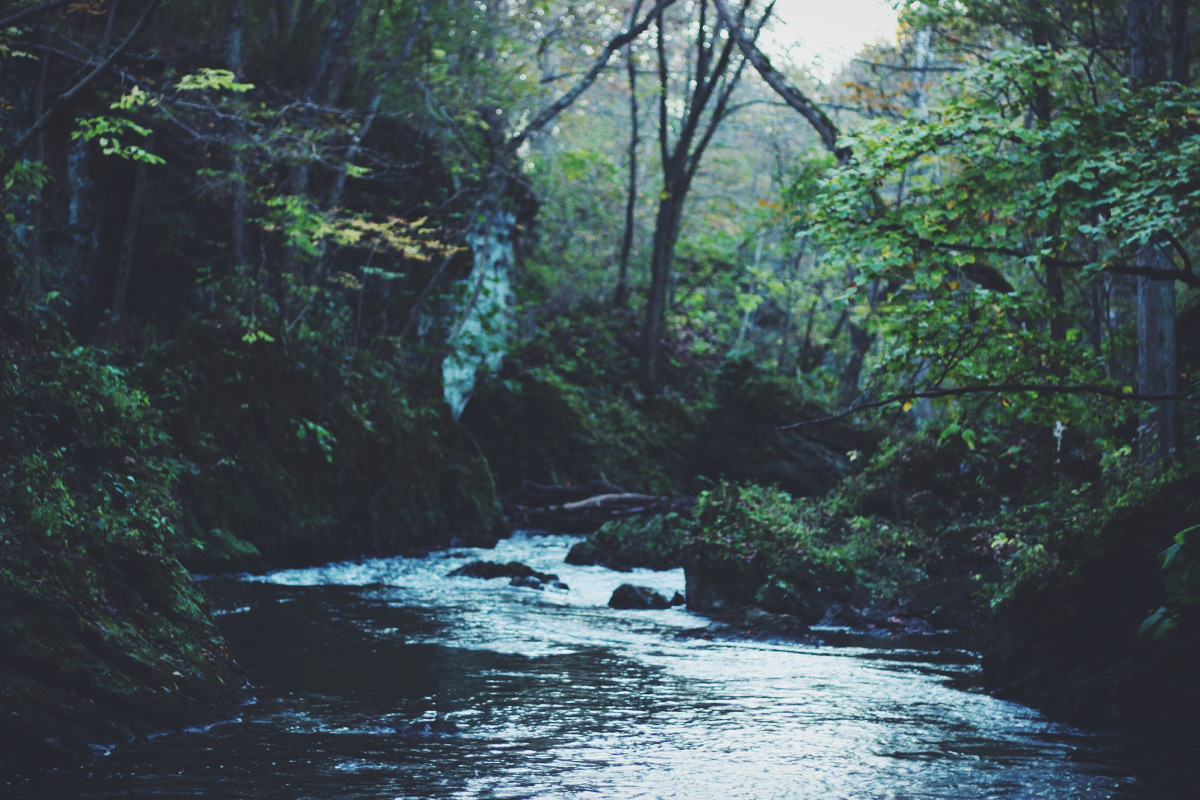
\includegraphics[width=\linewidth]{stream}
\caption{Legend (350 words max). Example legend text.}
\label{fig:stream}
\end{figure}

\begin{table}[ht]
\centering
\begin{tabular}{|l|l|l|}
\hline
Condition & n & p \\
\hline
A & 5 & 0.1 \\
\hline
B & 10 & 0.01 \\
\hline
\end{tabular}
\caption{\label{tab:example}Legend (350 words max). Example legend text.}
\end{table}

Figures and tables can be referenced in LaTeX using the ref command, e.g. Figure \ref{fig:stream} and Table \ref{tab:example}.
%REFERENCING________________________________________________________________________________________________________
\addcontentsline{toc}{section}{Bibliography} % add bibliography as a chapter

\bibliography{Zotero}        %use a bibtex bibliography file my_lib.bib
\bibliographystyle{plainnat}  %use the plain bibliography style

\end{document}
